\section{New Classification} \label{sec:Serotype_Classification}

\begin{figure}[!hbt]
    \centering
    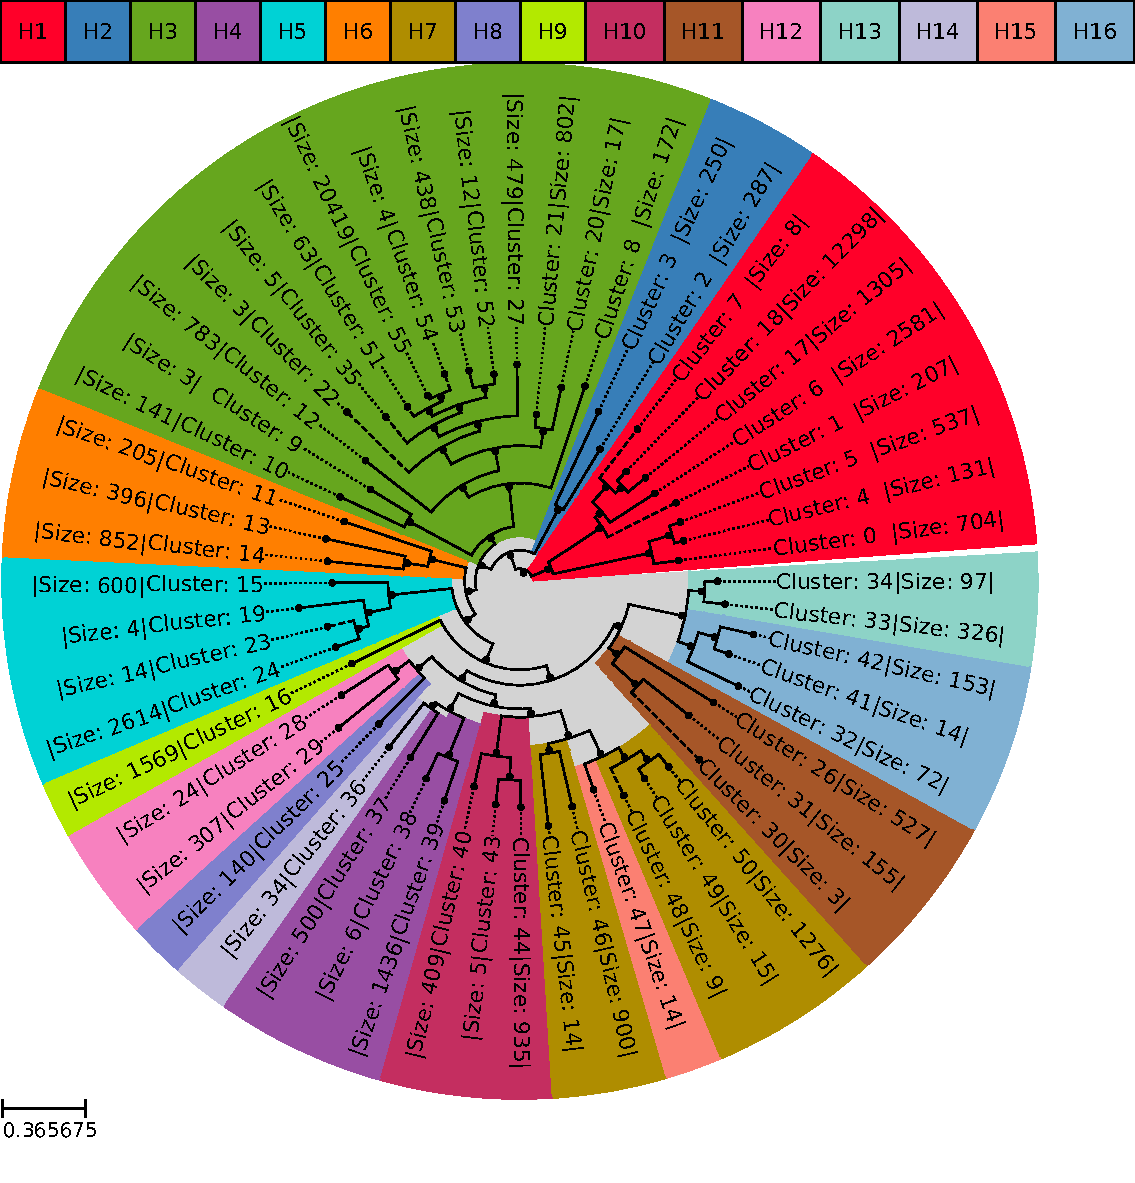
\includegraphics[width=\textwidth]{Results/Clustertree_Segment_4.pdf}
    \caption[]{}
    \label{fig:Result_Clustertree_Segment_4}
\end{figure}

Reannotation of the probably false annotated sequences in \autoref{fig:PCA_Clusteree_Knee_4} \textbf{\textsf{C}} as well as increasing of the components in \gls{PCA} successfully raised the accuracy of the pipeline. Clustering errors found in the previous section were resolved successfully as H13 and H16 are now completely divided, with the mentioned small but still present difference between these subtypes. Also all clusters of H3 are now present in direct connection to each other and no cluster not homogeneous for one subtype exist anymore. 

Thereby, new potential ways of \gls{IAV} clustering became possible. Resulting from the improved clustering of segment 4 a new classification involving 56 groups instead of 18 subtypes is proposed (\autoref{fig:Result_Clustertree_Segment_4}).
%neue classification vorschlagen blablabla
% vielleicht bisschen evolution black sea gull etc

By pairwise comparison of random 10 sequence samples of these groups the similarity inside these groups is described in \autoref{fig:Proof_Clustertree_Segment_4}. To avoid creating a bias, the result for accidental comparisons of sequences with the same accession are ignored and not considered in calculations of respective mean values.

\begin{figure}[!hbt]
    \centering
    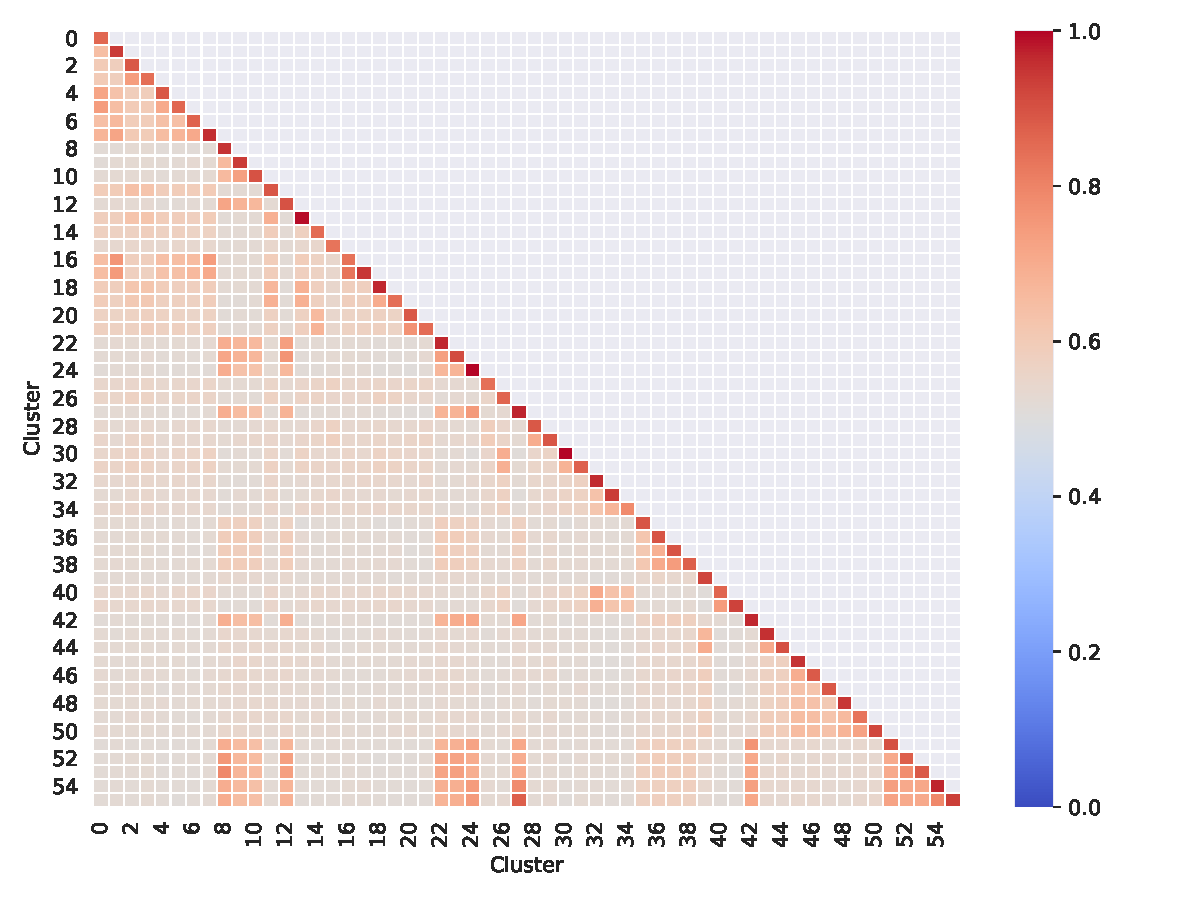
\includegraphics[width=\textwidth]{Results/Cluster_Difference_Segment_4.pdf}
    \caption[]{}
    \label{fig:Proof_Clustertree_Segment_4}
\end{figure}

All clusters in \autoref{fig:Proof_Clustertree_Segment_4} have the highest similarities with themselves and mostly high similarities with clusters of the same subtype. The cluster 0 as example, share some degree of sequence identity with other clusters stemming from the same subtype H1, as shown in \autoref{fig:Proof_Clustertree_Segment_4}. However, the highest similarity of around 90\% is only shared with other sequences of the cluster itself, which makes this cluster very self contained. 

Exceptions for the relative high similarity to other clusters of the same subtypes are the subtypes H7 and H15 with the clusters 45 to 50, as well as H4 and H14 with clusters 35 to 38. There was no clear separation performed as the clusters merge with other subtypes in higher tree nodes, although other clusters of the same subtype are still available (\autoref{fig:Result_Clustertree_Segment_4}). The similarities of these cluster are also high compared to the other subtype and indicate a relation neglected by the subtype classification. The almost uniform H7 sub tree of clusters 45, 46, 48, 49 and 50 is divided by the one and only cluster of subtype H15 cluster 47. When comparing the sequence similarities in \autoref{fig:Proof_Clustertree_Segment_4} the highest similarity persist inside the clusters themselves, but the cross similarities of cluster 45 and 46 to 47, 48, 49 and 50 are around 65\% without big difference between subtype H7 and H15.  

Similar colored trees and similarity matrix graphics, as well as tables containing sequence cluster assignment and the tables containing the values used to create the graphics are present in the \autoref{chap:Appendix}. Hereby new classifications for all segments based on k-mer frequency is proposed, containing 28 groups for segment one, 28 for two, 29 for three, the shown 57 for segment 4, 26 for five, 40 for six, 30 for seven and 24 groups for segment eight. 

The groups of the segments one to three, five, seven and eight share by far more overall similarity therefore less clusters were created. Still the similarity inside the clusters themselves is higher than the cross similarity and thereby solid clustering by the proposed clustering method was possible despite the overall higher similarity (\autoref{chap:Appendix}). 

Since exhaustion of the available time frame of this project, no further analysis were made, posterior to method and new classification proposal and the similarity matrix calculations as backup. Future research is thereby needed to further establish the classification by possible relations to specific strains or outbreaks of \gls{IAV}.